\chapter{General problem description}

In order to build the new rollator with the capability of giving directions to
the user and make him less ascared of unfamiliar places there are the following
two problems to solve.

\section{Indoor positioning system}
The first problem encountered is the localization of the elder inside a
building, and there are many solution available online which offer indoor 
GPS systems to try and buy.
However this platforms are based on a triangulation of Wi-fi signals united a
complete map of available hostspots.
\footnote{Further info at: 
\url{https://en.wikipedia.org/wiki/Wi-Fi_positioning_system}}
These kind of systems are full-stack solution to the problem and don't have the
necessary flexibility for the project's needs and, in addition, wi-fi hostspots 
aren't a possibility because the installation process would be a heavy burden
for user.
\newline
The team developing the project thought to use some sort of computer readable 
marker positioned inside the environment which contained the necessary information
and from this decision derived the usage of QR Codes, which I studied and
developed.

\newpage
\subsection{QR Code quick generalities}
A QRCode is foundamentally an image containing an encoded binary matrix of data which displays like:
\begin{figure}[hbt]
    \centering
    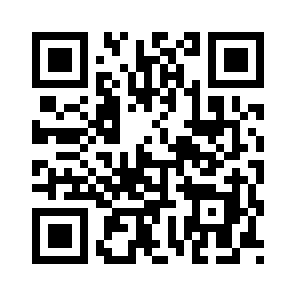
\includegraphics[scale=0.5]{img/qr.png}
\end{figure}

There are 41 versions of it and they differ from each other by their matrix 
module size which is fixed for each version and ranges from a minimum of 21x21 
to a maximum of 177x177. This allows to save up to 23648 bits.\footnote{with an L level or error correction}\footnote{complete table at: \url{http://www.qrcode.com/en/about/version.html}} 
\newline 
In addition, the encoding algorithm\footnote{ according to: \url{http://raidenii.net/files/datasheets/misc/qr_code.pdf}} offers the opportunity of error correction through the usage of Reed-Solomon codes.
These codes are also stored inside the QR Code and the there are four levels of error recovering which can be choosen by the user according to the operating environment.
In fact, each level increases its capability of restoring data but also require more space on the QR Code's matrix in order to work. 
\newpage
To simplify the above description here's a summarying table:
\begin{figure}[hbt]
    \centering
    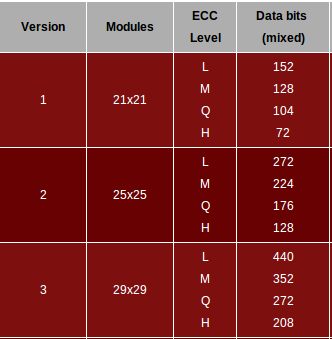
\includegraphics[scale=0.9]{img/qrversion.png}
\end{figure}


   













  
